\documentclass[acmtog,screen]{acmart}

\setcopyright{none}
\settopmatter{printacmref=false}
\renewcommand\footnotetextcopyrightpermission[1]{}

% Course/project metadata.
\acmConference[CS284A Spring 2026]{CS284A Final Project Milestone}{April 2026}{UC Berkeley}

% SIGGRAPH-style papers often use author-year citations.


\newcommand{\resimg}[1]{%
  \includegraphics[height=0.17\textheight,keepaspectratio]{#1}%
}

\begin{document}

\title{Fifty Shades of Cel: Milestone Report}

\author{Kevin Frans}
\affiliation{%
  \institution{University of California, Berkeley}
  \country{USA}
}
\email{kvfrans@berkeley.edu}

\author{Qijun Li}
\affiliation{%
  \institution{University of California, Berkeley}
  \country{USA}
}
\email{qijun.li@berkeley.edu}

\author{Shaoyi Wang}
\affiliation{%
  \institution{University of California, Berkeley}
  \country{USA}
}
\email{shaoyiwang@berkeley.edu}

\author{Tao Sun}
\affiliation{%
  \institution{University of California, Berkeley}
  \country{USA}
}
\email{tao_sun@berkeley.edu}

\renewcommand{\shortauthors}{Frans et al.}

\begin{abstract}
We present the milestone progress for Fifty Shades of Cel, a real-time non-photorealistic rendering pipeline for 2D/3D hybrid cel shading. Built on top of the HW4 cloth simulator's OpenGL framework, our system implements a two-pass rendering pipeline: a cel shading pass that computes quantized lighting bands with pattern textures, followed by a fullscreen post-process edge pass that detects silhouettes and feature lines from depth and normal buffers. We also provide a live GUI for interactive parameter tuning and shader export to Unity HLSL.
\end{abstract}

\keywords{cel shading, non-photorealistic rendering, real-time rendering, toon shading, stylized rendering}

\maketitle

\section{Introduction}

Cel shading, or toon shading, is a non-photorealistic rendering technique that makes 3D graphics appear flatter and more illustration-like rather than photorealistic~\cite{celshading}. This style is commonly used in stylized games and animated films because it combines the flexibility of 3D geometry with visual features associated with 2D animation, such as sharp silhouettes, discrete lighting regions, and simplified material appearance.

Our project, \textit{Fifty Shades of Cel}, explores a 2D/3D hybrid cel-shading pipeline built on top of the HW4 cloth simulator's OpenGL framework. The goal is to render dynamic 3D scenes with stylized outlines, flat color regions, texture-based shadow patterns, and interactive control over shader parameters.

At the milestone stage, we have implemented a two-pass rendering pipeline: a cel-shading pass that writes color, depth, and normal buffers, followed by a fullscreen post-process edge pass that detects silhouettes and feature lines from screen-space depth and normal discontinuities. We have also added live GUI controls for tuning the shader and an export path to Unity HLSL.

\section{Technical Approach}

Our implementation is organized as a two-pass rendering pipeline with interactive parameter control, as described in the following subsections.

\subsection{Rendering Pipeline Overview}

Our system uses a two-pass rendering pipeline. In the first pass, the scene is rendered into an offscreen framebuffer (FBO) that stores color, normal, and depth buffers using the cel shader. In the second pass, a fullscreen edge shader reads these buffers and composites detected outlines over the cel-shaded result.

\subsection{Cel Shader}

The cel fragment shader performs the main toon-shading computation. It first samples a pattern texture in UV space, tiled by a configurable scale parameter. It then computes $N \cdot L$ from the world-space normal and light direction, remaps this lighting value using a dark threshold, and quantizes it into discrete shadow bands using \texttt{floor()}. The shader applies the pattern texture to dark bands, modulated by a shadow-strength parameter, and adds a highlight band above a separate bright threshold. The pass outputs both the final cel-shaded color and an encoded normal buffer for the later edge pass.

\subsection{Edge Detection}

The fullscreen edge shader runs as a post-processing pass over the FBO outputs. For each pixel, it samples neighboring depth values to detect outer silhouettes and object-background boundaries, and samples neighboring normals to detect internal feature lines such as folds and creases. The resulting edge mask is composited over the color buffer from the first pass.

\subsection{GUI and Parameter Control}

All cel-shading parameters are exposed through a live GUI with per-frame updates. These include base, dark, and bright colors; dark and bright thresholds; shadow strength; highlight strength; number of bands; pattern texture scale; and light direction. This makes it possible to tune the final visual style interactively without recompiling the shader.

The current implementation also supports saving and loading cel-shading presets. In addition, the tuned parameters can be exported as Unity HLSL shader files, which provides a path for transferring the look from the simulator to a Unity material.

\subsection{Scene and Lighting Support}

The pipeline supports rendering multiple overlapping objects with correct depth compositing. Rigid geometry (spheres, planes, cubes constructed from individual faces) and deformable cloth meshes can coexist in the same scene. We added UV math corrections to ensure pattern textures scale correctly on planar geometry.

For lighting, the system supports both directional and point light sources. Point lights can be set to orbit the scene automatically, which is useful for previewing how the discrete shading bands respond to changing light directions. The light type and parameters are controllable through the GUI.

\section{Evaluation Plan}

We plan to evaluate our system along three axes:

\textbf{Visual quality.} We will compare our cel-shaded output against standard Phong shading on the same scenes, and conduct ablation studies by incrementally enabling each pipeline component (cel shading only, edge detection only, full pipeline) to verify each component's individual contribution. Figures~\ref{fig:edge_ablation} and~\ref{fig:bands} demonstrate early examples of this approach.

\textbf{Performance.} We will measure frame time and frame rate across scenes of increasing triangle count and object complexity, and report the per-pass overhead (cel shading pass vs. edge detection pass) relative to the baseline Phong renderer.

\textbf{Flexibility.} We will demonstrate parameter tunability by rendering galleries with varying band counts, edge thicknesses, color palettes, and light configurations, showing that the pipeline generalizes across different scenes and art styles.

\section{Preliminary Results}

Our pipeline is functional and produces cel-shaded renderings across several scene configurations.

\begin{figure}[htbp]
  \centering
  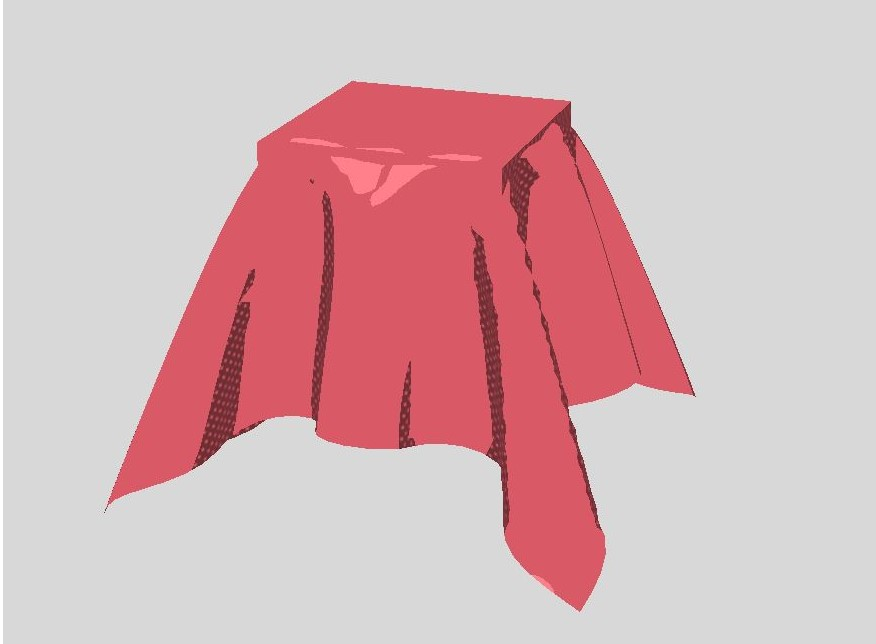
\includegraphics[width=0.48\linewidth]{figures/edge_off_cube.JPG}
  \hfill
  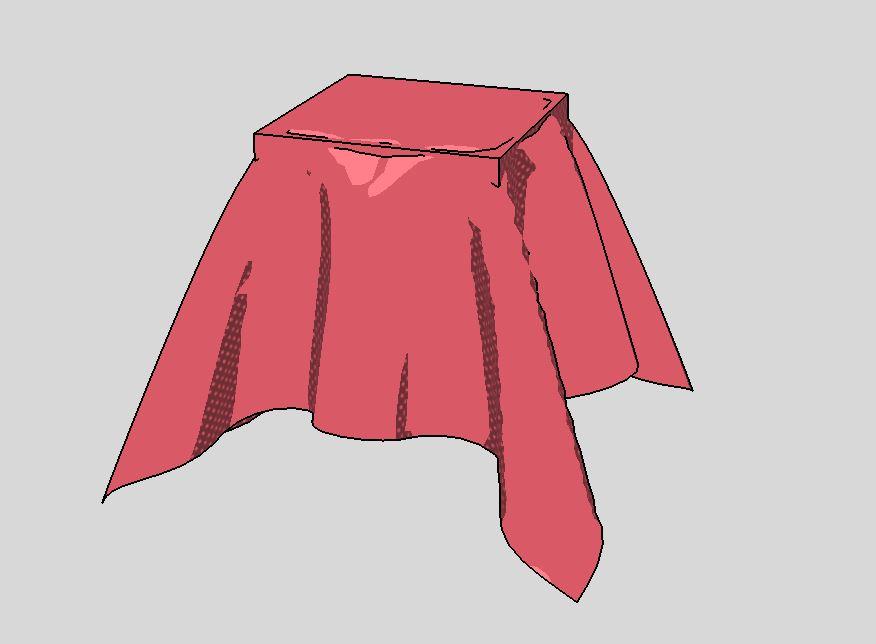
\includegraphics[width=0.48\linewidth]{figures/edge_on_cube.JPG}
  \caption{Edge detection ablation. Left: cel shading only, with edge pass disabled. Right: full pipeline with screen-space edge detection enabled, capturing both silhouette outlines and internal fold lines on the cloth.}
  \Description{Side-by-side comparison of cloth draped over a cube, without and with edge detection.}
  \label{fig:edge_ablation}
\end{figure}

\vspace{-10pt}
\begin{figure}[htbp]
  \centering
  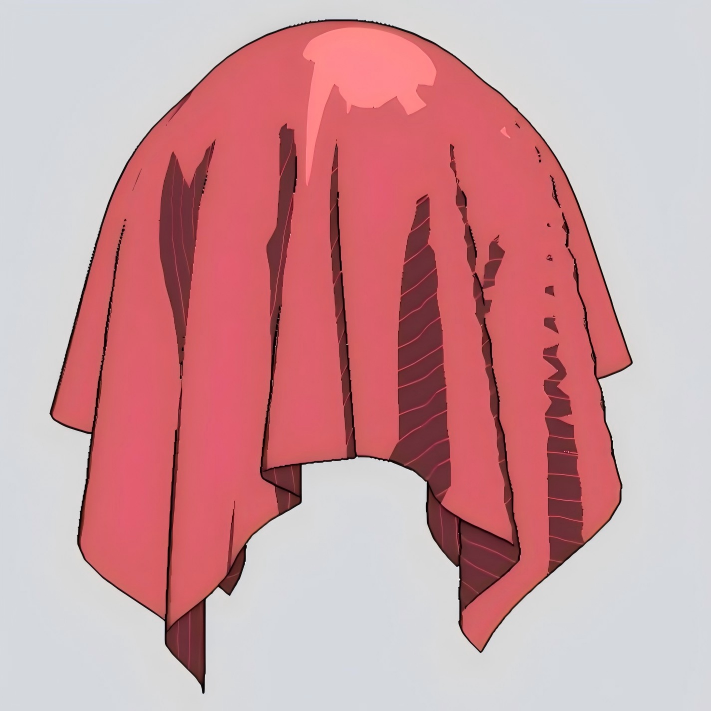
\includegraphics[width=0.32\linewidth]{figures/sphere_b1.png}
  \hfill
  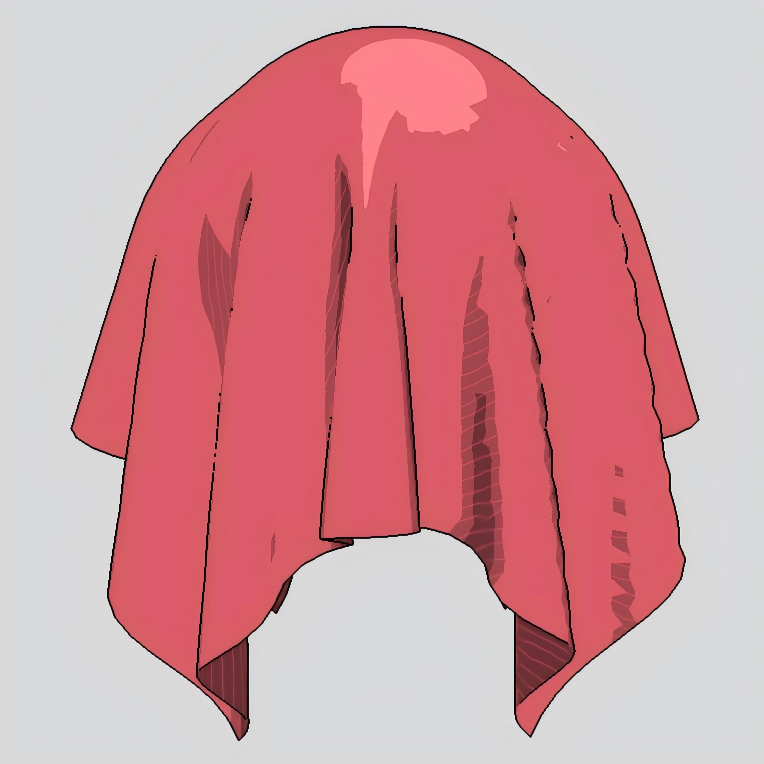
\includegraphics[width=0.32\linewidth]{figures/sphere_b2.png}
  \hfill
  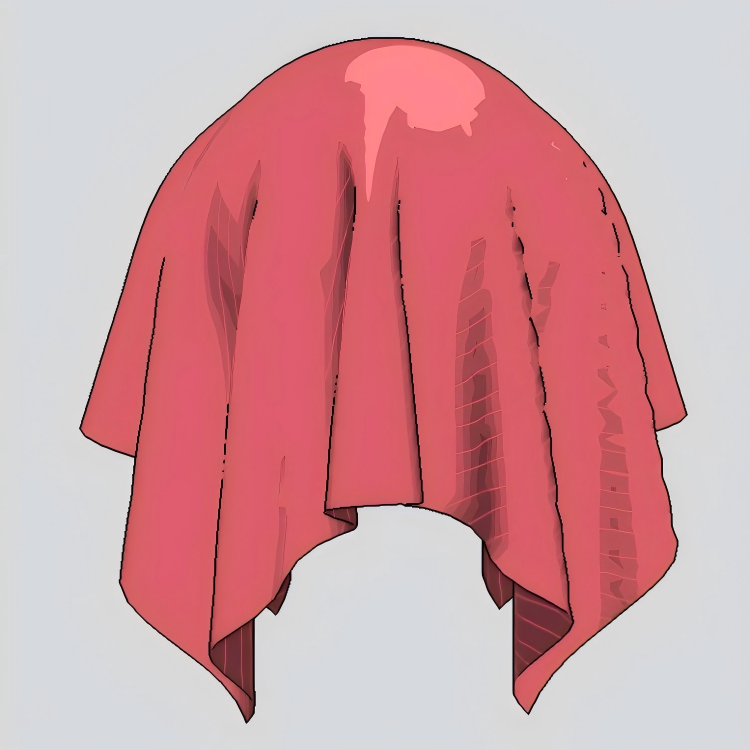
\includegraphics[width=0.32\linewidth]{figures/sphere_b4.png}
  \caption{Effect of varying the number of discrete lighting bands. From left to right: 1 band, 2 bands, and 4 bands. Increasing the band count introduces finer gradations in the shading while preserving the flat, stylized appearance.}
  \Description{Three renderings of cloth on a cube with 1, 2, and 4 lighting bands.}
  \label{fig:bands}
\end{figure}

\vspace{-10pt}
\begin{figure}[htbp]
  \centering
  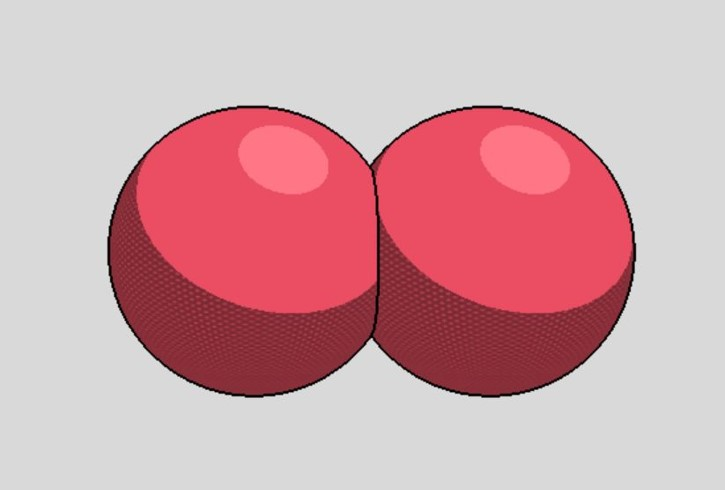
\includegraphics[width=0.48\linewidth]{figures/overlap_sphere.JPG}
  \hfill
  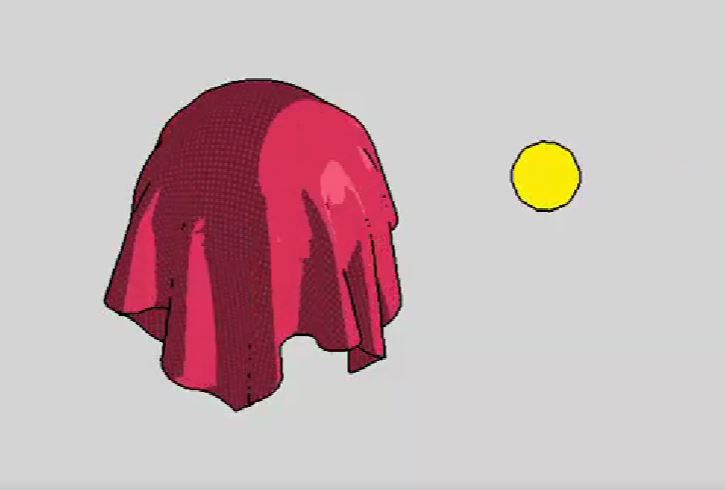
\includegraphics[width=0.48\linewidth]{figures/cube_light.JPG}
  \caption{Left: overlapping spheres with correct depth compositing and edge detection at object boundaries. Right: cloth scene with an animated orbiting point light source.}
  \Description{Overlapping spheres and a cloth scene with point light.}
  \label{fig:scenes}
\end{figure}

The system supports multiple overlapping objects with correct depth compositing and edge detection. Scenes can include both rigid geometry (spheres, planes, cubes) and deformable cloth meshes. Point lights with animated orbiting are supported, and all shading parameters can be adjusted interactively through the GUI.


\section{Progress and Updated Plan}

Our original proposal planned to complete edge detection and basic lighting by Week 2. At the milestone stage, the full two-pass pipeline is implemented and functional: the first pass performs cel shading with quantized lighting bands and pattern textures, while the second pass performs screen-space edge detection using depth and normal buffers. We have also implemented several features that support our planned final system, including multiple overlapping objects, point lights with animation, UV-corrected pattern scaling for planar geometry, a live GUI for shader parameters, and Unity HLSL export.

For the remaining two weeks, we plan to: (1) add shadow rendering; (2) test on more complex scenes with additional geometry and light configurations; (3) conduct performance benchmarking by measuring frame time across scenes of increasing triangle count; (4) implement stretch goals such as stylized shadow effects, additional art-style presets, and Blender integration if time permits; and (5) write the final paper and record the project video.

\section{References}

\begin{thebibliography}{9}

\bibitem{celshading}
Wikipedia contributors.
\textit{Cel shading}.
Wikipedia.
Available at: \url{https://en.wikipedia.org/wiki/Cel_shading}

\bibitem{toonTutorial}
Ned Makes Games.
\textit{Cel Shading Tutorial}.
YouTube.
Available at: \url{https://www.youtube.com/watch?v=dzItGHyteng}

\bibitem{stylizedTutorial}
Ned Makes Games.
\textit{Stylized Rendering Tutorial}.
YouTube.
Available at: \url{https://www.youtube.com/watch?v=s8N00rjil_4}

\bibitem{babylonOutline}
Babylon.js Forum.
\textit{How can I create a beautiful outline for meshes aka cell shading?}
Available at: \url{https://forum.babylonjs.com/t/how-can-i-create-a-beautiful-outline-for-meshes-aka-cell-shading/61556}

\bibitem{wireframe}
Freitas, C. M. D. S., Comba, J. L. D., and Nedel, L. P.
\textit{Texture-Based Wireframe Rendering}.
SIBGRAPI, 2010.
Available at: \url{http://sibgrapi.sid.inpe.br/col/sid.inpe.br/sibgrapi/2010/09.15.18.18/doc/texture-based_wireframe_rendering.pdf}

\bibitem{reyesDissertation}
Reyes Luque, R.
\textit{Cell-Shading Dissertation}.
2012.
Available at: \url{https://raulreyesfinalproject.wordpress.com/wp-content/uploads/2012/12/dissertation_cell-shading-raul_reyes_luque.pdf}

\bibitem{projectRepo}
Frans, K., Li, Q., Wang, S., and Sun, T.
\textit{CS284A\_50CelShades Project Repository}.
Available at: \url{https://github.com/LupoSun/CS284A_50CelShades}

\end{thebibliography}

\end{document}